\section{Thực nghiệm và đánh giá}
\label{sec:thuc_nghiem}

Chương này so sánh các cấu hình mô hình, đánh giá hai cách chuẩn hóa kích thước ảnh và phân tích những lỗi thường gặp. Các bảng ghi rõ tập dữ liệu dùng để tính chỉ số.

\subsection{Chỉ số đánh giá và lý do lựa chọn}
\label{sec:metrics}

Với mỗi lớp $k$, nhóm xem lớp đó là lớp dương và năm lớp còn lại là lớp âm. Từ ma trận nhầm lẫn (confusion matrix), nhóm đếm $TP_k$ là số ảnh lớp $k$ được phân loại đúng, $FP_k$ là số ảnh của lớp khác bị phân loại thành lớp $k$ và $FN_k$ là số ảnh lớp $k$ bị phân loại thành lớp khác. Ba chỉ số theo lớp được tính như sau.
\begin{align}
  \text{Precision}_k &= \frac{TP_k}{TP_k + FP_k}, \\
  \text{Recall}_k &= \frac{TP_k}{TP_k + FN_k}, \\
  F1_k &= \frac{2 \cdot \text{Precision}_k \cdot \text{Recall}_k}{\text{Precision}_k + \text{Recall}_k} .
\end{align}
Precision cho biết tỷ lệ dự đoán đúng trong số các ảnh được gán vào một lớp. Recall cho biết tỷ lệ dự đoán đúng trong số các ảnh thực sự thuộc lớp đó. Ví dụ, recall của lớp \texttt{pistol} là tỷ lệ ảnh súng ngắn được phân loại đúng. F1 là trung bình điều hòa của precision và recall.

Nhóm báo cáo các chỉ số tổng hợp sau.

\begin{itemize}
  \item \textbf{Macro-F1.} Trung bình cộng của $F1_k$ trên sáu lớp. Lớp \texttt{tarjeta} (74 ảnh trong tập test) có trọng số bằng lớp \texttt{pistol} (662 ảnh trong tập test). Nhóm dùng macro-F1 làm chỉ số chính khi so sánh các cấu hình trên tập validation.
  \item \textbf{Độ chính xác chung (accuracy).} Tỷ lệ ảnh được phân loại đúng. Để đối chiếu, bộ phân loại luôn dự đoán lớp \texttt{pistol} sẽ đạt 41,7\% trên tập test.
  \item \textbf{Độ chính xác cân bằng (balanced accuracy).} Trung bình cộng của recall theo lớp, với trọng số như nhau cho sáu lớp.
  \item \textbf{Weighted-F1.} Trung bình của $F1_k$ với trọng số tỷ lệ thuận với số ảnh của từng lớp. Khi weighted-F1 cao hơn macro-F1, việc tăng trọng số cho các lớp có nhiều ảnh làm điểm tổng hợp cao hơn. Kết quả theo lớp cho biết cụ thể lớp nào có F1 cao hoặc thấp.
  \item \textbf{Hệ số tương quan Matthews (MCC).} Chỉ số này đo mức độ tương ứng giữa nhãn dự đoán và nhãn thực, với giá trị từ $-1$ đến $1$. Giá trị 1 tương ứng với dự đoán hoàn toàn đúng.
  \item \textbf{Log-loss và ROC-AUC.} Nhóm báo cáo hai chỉ số này cho hồi quy logistic. Log-loss là trung bình của $-\log \hat{p}_{y_i}(\mathbf{x}_i)$ trên các ảnh được đánh giá. Mất mát tăng khi xác suất ước lượng cho nhãn đúng giảm. ROC-AUC là diện tích dưới đường cong ROC. Chỉ số này đo khả năng xếp hạng ảnh thuộc một lớp cao hơn ảnh thuộc các lớp còn lại theo xác suất ước lượng cho lớp đó. Nhóm tính ROC-AUC cho từng lớp rồi lấy trung bình trên sáu lớp.
\end{itemize}

Nhóm cũng gộp \texttt{pistol} và \texttt{knife} thành nhóm vũ khí, gộp bốn lớp còn lại thành nhóm đồ vật thông thường và tính hai tỷ lệ trên tập test.
\begin{itemize}
  \item \textbf{Tỷ lệ bỏ sót vũ khí.} Tỷ lệ ảnh bị phân loại thành đồ vật thông thường trong 1.053 ảnh vũ khí.
  \item \textbf{Tỷ lệ báo động nhầm.} Tỷ lệ ảnh bị phân loại thành vũ khí trong 535 ảnh đồ vật thông thường.
\end{itemize}
Khi tính hai tỷ lệ theo nhóm, ảnh dao bị phân loại thành súng ngắn vẫn thuộc nhóm vũ khí. Trường hợp này vẫn được tính là lỗi trong đánh giá sáu lớp.

\subsection{Cấu hình thực nghiệm}

\begin{itemize}
  \item \textbf{Dữ liệu.} Các mô hình dùng chung 6.361 ảnh trong tập train, 1.594 ảnh trong tập validation và 1.588 ảnh trong tập test (Bảng~\ref{tab:split}).
  \item \textbf{SVM.} Nhóm huấn luyện trên CPU của Kaggle cho cả hai nhánh \emph{direct} và \emph{padding}.
  \item \textbf{Hồi quy logistic.} Nhóm huấn luyện trên CPU của Google Colab, dùng nhánh \emph{padding}.
  \item \textbf{Phần mềm.} Nhóm dùng Python với scikit-learn, scikit-image, OpenCV và NumPy.
  \item \textbf{Giá trị khởi tạo ngẫu nhiên.} Chương trình chia dữ liệu, PCA ngẫu nhiên và SVM tuyến tính dùng giá trị khởi tạo bằng 42.
\end{itemize}

\subsection{Kết quả của SVM}

\subsubsection{Tinh chỉnh siêu tham số}
\label{sec:svm_tuning}

\paragraph{SVM tuyến tính.} Khi $C$ tăng từ 0,1 lên 100, macro-F1 trên tập validation thay đổi ít ở cả hai nhánh. Trong các giá trị khảo sát, $C = 0{,}001$ cho điểm cao nhất, với 0,6037 ở nhánh \emph{direct} và 0,5840 ở nhánh \emph{padding} (Bảng~\ref{tab:tune_linear}).

\begin{table}[H]
\centering
\caption{Macro-F1 của SVM tuyến tính trên tập validation theo $C$}
\label{tab:tune_linear}
\begin{tabular}{@{}lcccccc@{}}
\toprule
$C$ & 0,001 & 0,01 & 0,1 & 1 & 10 & 100 \\
\midrule
\emph{direct}  & \textbf{0,6037} & 0,6011 & 0,6010 & 0,6010 & 0,6010 & 0,6010 \\
\emph{padding} & \textbf{0,5840} & 0,5783 & 0,5755 & 0,5755 & 0,5748 & 0,5748 \\
\bottomrule
\end{tabular}
\end{table}

Giá trị $C$ có điểm cao nhất nằm ở biên dưới của dải khảo sát. Kết quả hiện có chưa cho biết liệu $C$ nhỏ hơn 0,001 có cải thiện điểm hay không.

\begin{figure}[H]
  \centering
  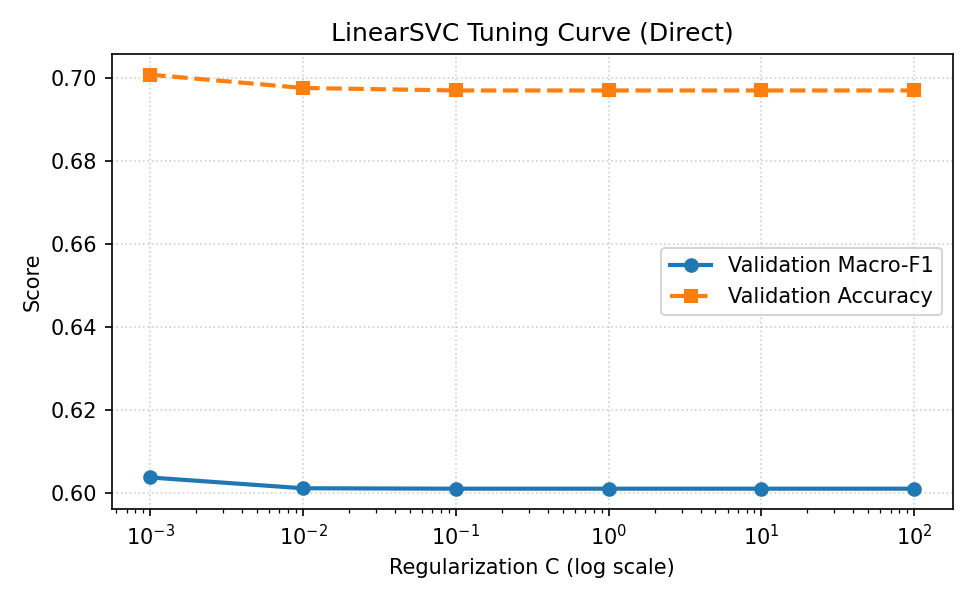
\includegraphics[width=0.7\textwidth]{val_curve_linearsvc_direct.png}
  \caption{Macro-F1 và accuracy trên tập validation của SVM tuyến tính (nhánh \emph{direct}) theo $C$}
  \label{fig:tune_linear}
\end{figure}

\paragraph{SVM RBF.} Trên nhánh \emph{direct}, các cấu hình dùng \texttt{gamma="scale"} đạt macro-F1 từ 0,6914 đến 0,7245 trên tập validation. Khi đặt $\gamma = 0{,}01$, macro-F1 là 0,0979 ở cả ba giá trị $C$ (Bảng~\ref{tab:tune_rbf}).

\begin{table}[H]
\centering
\caption{Macro-F1 của SVM RBF trên tập validation theo $C$ và $\gamma$ (nhánh \emph{direct})}
\label{tab:tune_rbf}
\begin{tabular}{@{}lccc@{}}
\toprule
 & $\gamma = \texttt{"scale"}$ & $\gamma = 0{,}01$ & $\gamma = 0{,}001$ \\
\midrule
$C = 1$  & 0,6914 & 0,0979 & 0,1422 \\
$C = 10$ & \textbf{0,7245} & 0,0979 & 0,1489 \\
$C = 50$ & 0,7244 & 0,0979 & 0,1489 \\
\bottomrule
\end{tabular}
\end{table}

Với $\gamma = 0{,}01$, độ chính xác 0,4159 bằng tỷ lệ ảnh \texttt{pistol} trong tập validation ($663 / 1.594$). Nếu bộ phân loại gán mọi ảnh vào lớp này, F1 của lớp \texttt{pistol} sẽ xấp xỉ 0,587, năm lớp còn lại có F1 bằng 0 và macro-F1 xấp xỉ 0,098. Hai chỉ số quan sát được phù hợp với trường hợp mọi ảnh đều bị gán vào lớp \texttt{pistol}.

Một cách giải thích là $\gamma = 0{,}01$ quá lớn so với thang khoảng cách sau PCA. Theo công thức~\eqref{eq:rbf}, khi tích của $\gamma$ và bình phương khoảng cách lớn, giá trị hàm nhân giữa hai vectơ tiến gần về 0. Chế độ \texttt{"scale"} đặt $\gamma$ theo phương sai của ma trận đầu vào (công thức~\eqref{eq:gammascale}) và cho macro-F1 cao hơn hai giá trị cố định đã thử.

\subsubsection{Kết quả trên tập test}

Bảng~\ref{tab:svm_test} trình bày kết quả trên tập test của bốn cấu hình SVM đã được chọn trên tập validation.

\begin{table}[H]
\centering
\caption{Kết quả của bốn cấu hình SVM trên tập test}
\label{tab:svm_test}
\small
\setlength{\tabcolsep}{4pt}
\begin{tabularx}{\linewidth}{@{}Xlccccr@{}}
\toprule
\textbf{Mô hình} & \textbf{Nhánh} & \textbf{Accuracy} &
\shortstack{\textbf{Balanced}\\\textbf{accuracy}} & \textbf{Macro-F1} &
\shortstack{\textbf{Weighted}\\\textbf{F1}} & \shortstack{\textbf{Thời gian}\\\textbf{(s)}} \\
\midrule
SVM tuyến tính \mbox{($C = 0{,}001$)} & \emph{direct}  & 0,7185 & 0,6125 & 0,6292 & 0,7140 & 179,1 \\
SVM tuyến tính \mbox{($C = 0{,}001$)} & \emph{padding} & 0,6751 & 0,5609 & 0,5745 & 0,6699 & 121,4 \\
SVM RBF \mbox{($C = 10$, \texttt{scale})} & \emph{direct}  & \textbf{0,8388} & \textbf{0,7345} & \textbf{0,7632} & \textbf{0,8341} & 4,8 \\
SVM RBF \mbox{($C = 10$, \texttt{scale})} & \emph{padding} & 0,8205 & 0,7253 & 0,7506 & 0,8164 & 5,9 \\
\bottomrule
\end{tabularx}
\end{table}

Hai kết quả chính liên quan đến mô hình và cách chuẩn hóa kích thước.

\begin{enumerate}
  \item \textbf{SVM RBF kết hợp PCA đạt điểm cao hơn SVM tuyến tính trên cả hai nhánh.} Trên nhánh \emph{direct}, macro-F1 là 0,763 so với 0,629, chênh 0,134. Độ chính xác lần lượt là 83,9\% và 71,9\%.
  \item \textbf{Nhánh \emph{direct} đạt macro-F1 cao hơn nhánh \emph{padding}.} Chênh lệch là 0,055 với SVM tuyến tính và 0,013 với SVM RBF. Mục~\ref{sec:discussion} trình bày các giả thuyết giải thích chênh lệch này.

\end{enumerate}
Thời gian trong bảng được đo ở bước huấn luyện cấu hình cuối cùng. Với SVM tuyến tính, phép đo gồm chuẩn hóa đặc trưng và huấn luyện bộ phân loại. Với SVM RBF, phép đo bắt đầu sau bước chuẩn hóa và chiếu PCA. Hai giá trị vì vậy có phạm vi đo khác nhau.


\subsection{Kết quả của hồi quy logistic}

\subsubsection{So sánh các biến thể trên tập validation}

Bảng~\ref{tab:lr_val} so sánh năm biến thể hồi quy logistic. Cột chênh lệch lấy macro-F1 trên tập train trừ macro-F1 trên tập validation và được dùng để nhận biết dấu hiệu quá khớp.

\begin{table}[H]
\centering
\caption{Các biến thể hồi quy logistic trên tập validation (nhánh \emph{padding}, $C = 1$)}
\label{tab:lr_val}
\small
\begin{tabularx}{\linewidth}{@{}Xccccc@{}}
\toprule
\textbf{Biến thể} & \shortstack{\textbf{Số đặc}\\\textbf{trưng}} &
\shortstack{\textbf{F1 huấn}\\\textbf{luyện}} & \shortstack{\textbf{F1 xác}\\\textbf{thực}} &
\shortstack{\textbf{Chênh}\\\textbf{lệch}} & \textbf{Log-loss} \\
\midrule
Mô hình cơ sở (L2)       & 26.244 & 1,000 & \textbf{0,591} & 0,409 & 2,10 \\
Lọc ANOVA + L2           &  8.000 & 1,000 & 0,541 & 0,459 & 2,90 \\
Lọc ANOVA + L2           &  3.000 & 1,000 & 0,470 & 0,530 & 3,22 \\
Lọc ANOVA + L2           &  1.000 & 0,849 & 0,392 & 0,457 & 2,57 \\
Lọc ANOVA + L1           &  8.000 & 1,000 & 0,558 & 0,442 & \textbf{1,52} \\
\bottomrule
\end{tabularx}
\end{table}

Mô hình cơ sở đạt macro-F1 cao nhất trên tập validation. Kết quả theo từng biến thể cho thấy bốn điểm.

\begin{itemize}
  \item \textbf{Chênh lệch giữa kết quả trên tập train và tập validation.} Bốn trong năm biến thể đạt macro-F1 xấp xỉ 1 trên tập train. Trên tập validation, macro-F1 của năm biến thể nằm trong khoảng 0,392 đến 0,591. Chênh lệch giữa hai tập cho thấy dấu hiệu quá khớp.
  \item \textbf{Giảm số đặc trưng bằng ANOVA.} Với điều chuẩn L2, macro-F1 trên tập validation lần lượt là 0,591 khi dùng toàn bộ đặc trưng và 0,541, 0,470, 0,392 khi giữ 8.000, 3.000 và 1.000 đặc trưng. Trong các cấu hình này, lọc ANOVA làm giảm macro-F1 và chênh lệch giữa hai tập vẫn lớn.
  \item \textbf{Kết hợp ANOVA với điều chuẩn L1.} Khi giữ cùng 8.000 đặc trưng, biến thể L1 đạt macro-F1 0,558, so với 0,541 của L2. Có 22.563 trong 48.000 hệ số khác 0 (47\%). Thuật toán SAGA chạm giới hạn 300 vòng lặp sau 1.422 giây (khoảng 24 phút) và chưa hội tụ.
  \item \textbf{Kết quả log-loss.} Biến thể ANOVA + L1 đạt log-loss 1,52, thấp nhất trong năm biến thể trên tập validation.
\end{itemize}

\begin{figure}[H]
  \centering
  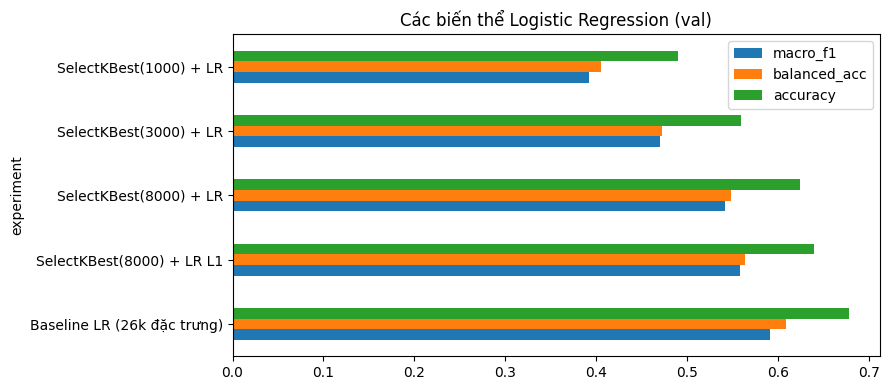
\includegraphics[width=0.85\textwidth]{lr_variants_val.png}
  \caption{Macro-F1, balanced accuracy và accuracy của các biến thể hồi quy logistic trên tập validation}
  \label{fig:lr_variants}
\end{figure}

\subsubsection{Kết quả trên tập test}

Nhóm chọn mô hình cơ sở vì mô hình này đạt macro-F1 cao nhất trên tập validation (0,591). Trên tập test, macro-F1 đạt 0,577 (Bảng~\ref{tab:lr_test}).

\begin{table}[H]
\centering
\caption{Kết quả của hồi quy logistic cơ sở trên tập test}
\label{tab:lr_test}
\small
\setlength{\tabcolsep}{4pt}
\begin{tabular}{@{}ccccccc@{}}
\toprule
\textbf{Accuracy} & \shortstack{\textbf{Balanced}\\\textbf{accuracy}} &
\textbf{Macro-F1} & \shortstack{\textbf{Weighted}\\\textbf{F1}} &
\textbf{MCC} & \textbf{Log-loss} & \textbf{ROC-AUC} \\
\midrule
0,6776 & 0,5857 & 0,5767 & 0,6818 & 0,5686 & 2,173 & 0,8752 \\
\bottomrule
\end{tabular}
\end{table}

Hồi quy logistic cơ sở đạt ROC-AUC trung bình 0,875. Từ các xác suất đã lưu, nhóm xếp hạng sáu lớp cho từng ảnh trên tập test. Trong 512 ảnh bị phân loại sai, nhãn đúng đứng thứ hai hoặc thứ ba ở 342 ảnh (66,8\%).

\paragraph{Xác suất ước lượng ở các dự đoán sai.} Trong 512 ảnh bị phân loại sai trên tập test, 263 ảnh (51\%) được gán xác suất trên 0,9 cho nhãn dự đoán sai. Xác suất trung bình của nhãn được dự đoán là 0,835 ở nhóm dự đoán sai và 0,953 ở nhóm dự đoán đúng. Vì nhiều dự đoán sai vẫn có xác suất ước lượng cao, cần đánh giá riêng mức thay đổi của tỷ lệ bỏ sót và báo động nhầm trước khi chọn ngưỡng cảnh báo.

\begin{figure}[H]
  \centering
  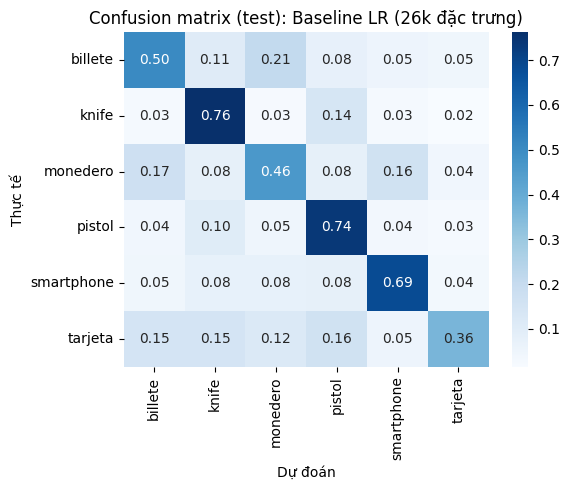
\includegraphics[width=0.6\textwidth]{lr_cm_test.png}
  \caption{Ma trận nhầm lẫn chuẩn hóa theo hàng của hồi quy logistic trên tập test}
  \label{fig:lr_cm}
\end{figure}

\subsection{So sánh các mô hình}
\label{sec:compare}

\subsubsection{So sánh tổng thể}

Để đối chiếu các mô hình dưới cùng một cách chuẩn hóa kích thước, nhóm so sánh ba cấu hình trên nhánh \emph{padding}. Bảng~\ref{tab:compare} cũng trình bày kết quả của hai biến thể SVM trên nhánh \emph{direct}. SVM được tinh chỉnh siêu tham số, còn hồi quy logistic dùng $C = 1$.

\begin{table}[H]
\centering
\caption{So sánh các mô hình trên tập test}
\label{tab:compare}
\small
\begin{tabularx}{\linewidth}{@{}lXcccc@{}}
\toprule
\textbf{Nhánh} & \textbf{Mô hình} & \textbf{Accuracy} &
\shortstack{\textbf{Balanced}\\\textbf{accuracy}} & \textbf{Macro-F1} &
\shortstack{\textbf{Weighted}\\\textbf{F1}} \\
\midrule
\multirow{3}{*}{\emph{padding}}
  & Hồi quy logistic ($C = 1$)  & 0,6776 & 0,5857 & 0,5767 & 0,6818 \\
  & SVM tuyến tính ($C = 0{,}001$) & 0,6751 & 0,5609 & 0,5745 & 0,6699 \\
  & SVM RBF                     & 0,8205 & 0,7253 & 0,7506 & 0,8164 \\
\midrule
\multirow{2}{*}{\emph{direct}}
  & SVM tuyến tính ($C = 0{,}001$) & 0,7185 & 0,6125 & 0,6292 & 0,7140 \\
  & SVM RBF                     & \textbf{0,8388} & \textbf{0,7345} & \textbf{0,7632} & \textbf{0,8341} \\
\bottomrule
\end{tabularx}
\end{table}

Trên nhánh \emph{padding}, hồi quy logistic và SVM tuyến tính đạt macro-F1 lần lượt là 0,577 và 0,575. SVM RBF kết hợp PCA đạt 0,751, cao hơn khoảng 0,17 điểm so với hai cấu hình tuyến tính. Sự khác biệt giữa các cấu hình còn bao gồm bước PCA, hàm mất mát và cách chọn mức điều chuẩn, nên phép so sánh này chưa xác định được đóng góp riêng của từng yếu tố.

\subsubsection{So sánh theo từng lớp}

\begin{table}[H]
\centering
\caption{F1 và recall theo từng lớp trên tập test}
\label{tab:per_class}
\small
\setlength{\tabcolsep}{4pt}
\begin{tabular}{@{}lr cc cc cc@{}}
\toprule
 & & \multicolumn{2}{c}{\textbf{Hồi quy logistic}} & \multicolumn{2}{c}{\textbf{SVM tuyến tính}} & \multicolumn{2}{c}{\textbf{SVM RBF}} \\
 & & \multicolumn{2}{c}{(\emph{padding})} & \multicolumn{2}{c}{(\emph{direct})} & \multicolumn{2}{c}{(\emph{direct})} \\
\cmidrule(lr){3-4}\cmidrule(lr){5-6}\cmidrule(lr){7-8}
\textbf{Lớp} & \textbf{Số ảnh} & F1 & Recall & F1 & Recall & F1 & Recall \\
\midrule
\texttt{pistol}     & 662 & 0,779 & 0,739 & 0,791 & 0,816 & \textbf{0,890} & \textbf{0,950} \\
\texttt{knife}      & 391 & 0,737 & 0,762 & 0,758 & 0,767 & \textbf{0,888} & \textbf{0,877} \\
\texttt{smartphone} & 197 & 0,675 & 0,685 & 0,704 & 0,695 & \textbf{0,830} & \textbf{0,756} \\
\texttt{monedero}   & 135 & 0,428 & 0,459 & 0,524 & 0,526 & \textbf{0,661} & \textbf{0,548} \\
\texttt{billete}    & 129 & 0,469 & 0,504 & 0,554 & 0,519 & \textbf{0,699} & \textbf{0,775} \\
\texttt{tarjeta}    &  74 & 0,372 & 0,365 & 0,444 & 0,351 & \textbf{0,612} & \textbf{0,500} \\
\bottomrule
\end{tabular}
\end{table}

Trong ba cấu hình được trình bày ở Bảng~\ref{tab:per_class}, SVM RBF trên nhánh \emph{direct} đạt F1 và recall cao nhất ở cả sáu lớp. Với cấu hình này, F1 của lớp \texttt{pistol} và \texttt{knife} lần lượt là 0,890 và 0,888, trong khi F1 của \texttt{tarjeta} và \texttt{monedero} lần lượt là 0,612 và 0,661. Hai lớp có F1 thấp hơn cũng có ít ảnh trong tập train hơn hai lớp vũ khí.

\subsubsection{So sánh theo mục đích giám sát an ninh}

Bảng~\ref{tab:weapon} trình bày kết quả sau khi gộp sáu lớp thành hai nhóm theo Mục~\ref{sec:metrics}. Nhóm đếm trực tiếp từ kết quả dự đoán của hai mô hình tuyến tính. Với SVM RBF, số đếm được suy ra từ các tỷ lệ đã làm tròn trong Hình~\ref{fig:cm_rbf}, nên được báo cáo dưới dạng xấp xỉ.

\begin{table}[H]
\centering
\caption{Tỷ lệ bỏ sót vũ khí và báo động nhầm trên tập test}
\label{tab:weapon}
\small
\begin{tabular}{@{}lcc@{}}
\toprule
\textbf{Mô hình} & \shortstack{\textbf{Bỏ sót vũ khí}\\(trên 1.053 ảnh)} &
\shortstack{\textbf{Báo động nhầm}\\(trên 535 ảnh)} \\
\midrule
Hồi quy logistic (\emph{padding})  & 142 ảnh (13,5\%) & 100 ảnh (18,7\%) \\
SVM tuyến tính (\emph{padding})   &  92 ảnh (8,7\%)  & 159 ảnh (29,7\%) \\
SVM tuyến tính (\emph{direct})    &  77 ảnh (7,3\%)  & 128 ảnh (23,9\%) \\
SVM RBF (\emph{direct})           & khoảng 18 ảnh (1,7\%) & khoảng 98 ảnh (18,3\%) \\
\bottomrule
\end{tabular}
\end{table}

Trên nhánh \emph{direct}, tỷ lệ bỏ sót vũ khí của SVM RBF là khoảng 1,7\%, so với 7,3\% của SVM tuyến tính. Tỷ lệ báo động nhầm của các cấu hình trong bảng nằm trong khoảng 18\% đến 30\%. Với SVM RBF, ví và điện thoại chiếm phần lớn số ảnh bị phân loại nhầm thành vũ khí, lần lượt khoảng 34 và 28 ảnh. Các tỷ lệ được tính trên ảnh đã cắt quanh vật thể.

\begin{figure}[H]
  \centering
  \begin{subfigure}{0.49\textwidth}
    \centering
    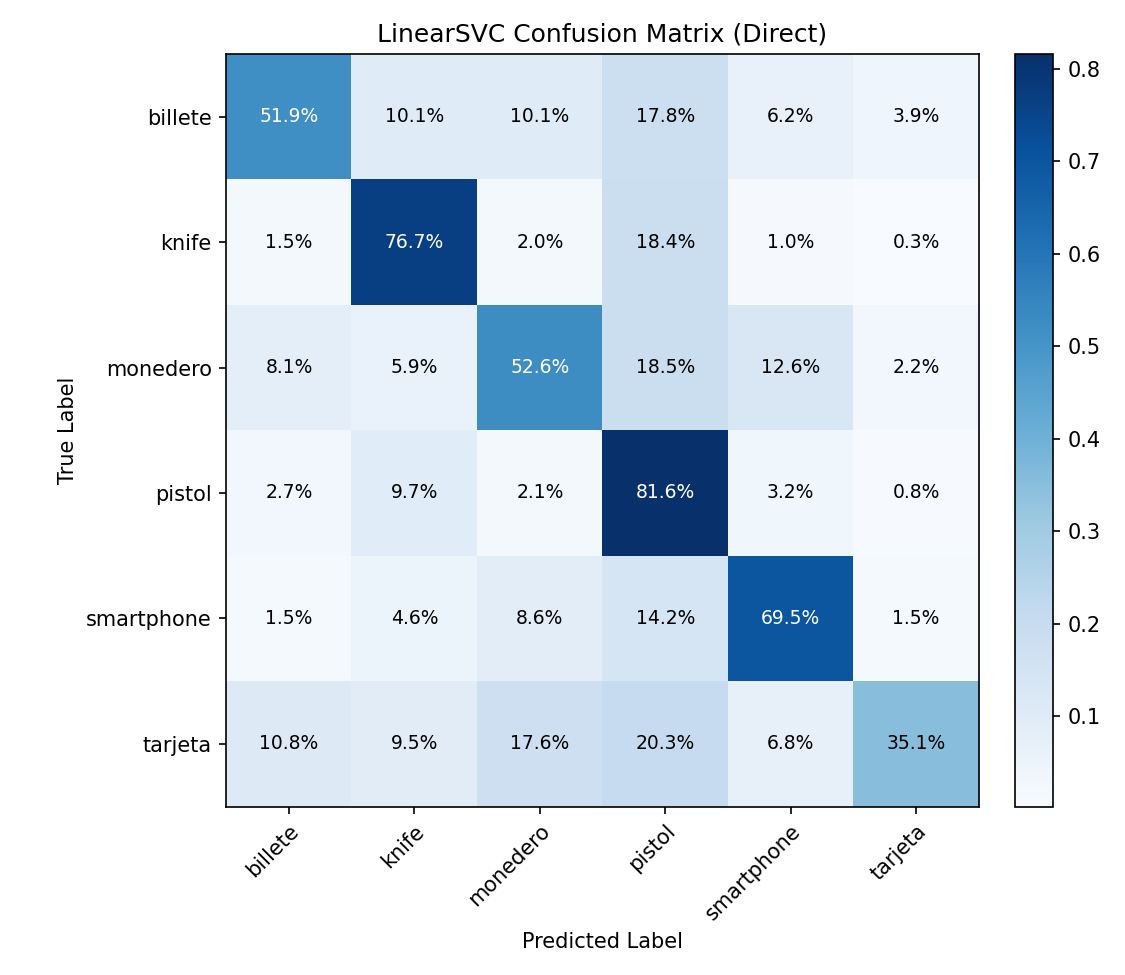
\includegraphics[width=\textwidth]{confusion_matrix_linear_direct.png}
    \caption{SVM tuyến tính}
  \end{subfigure}
  \hfill
  \begin{subfigure}{0.49\textwidth}
    \centering
    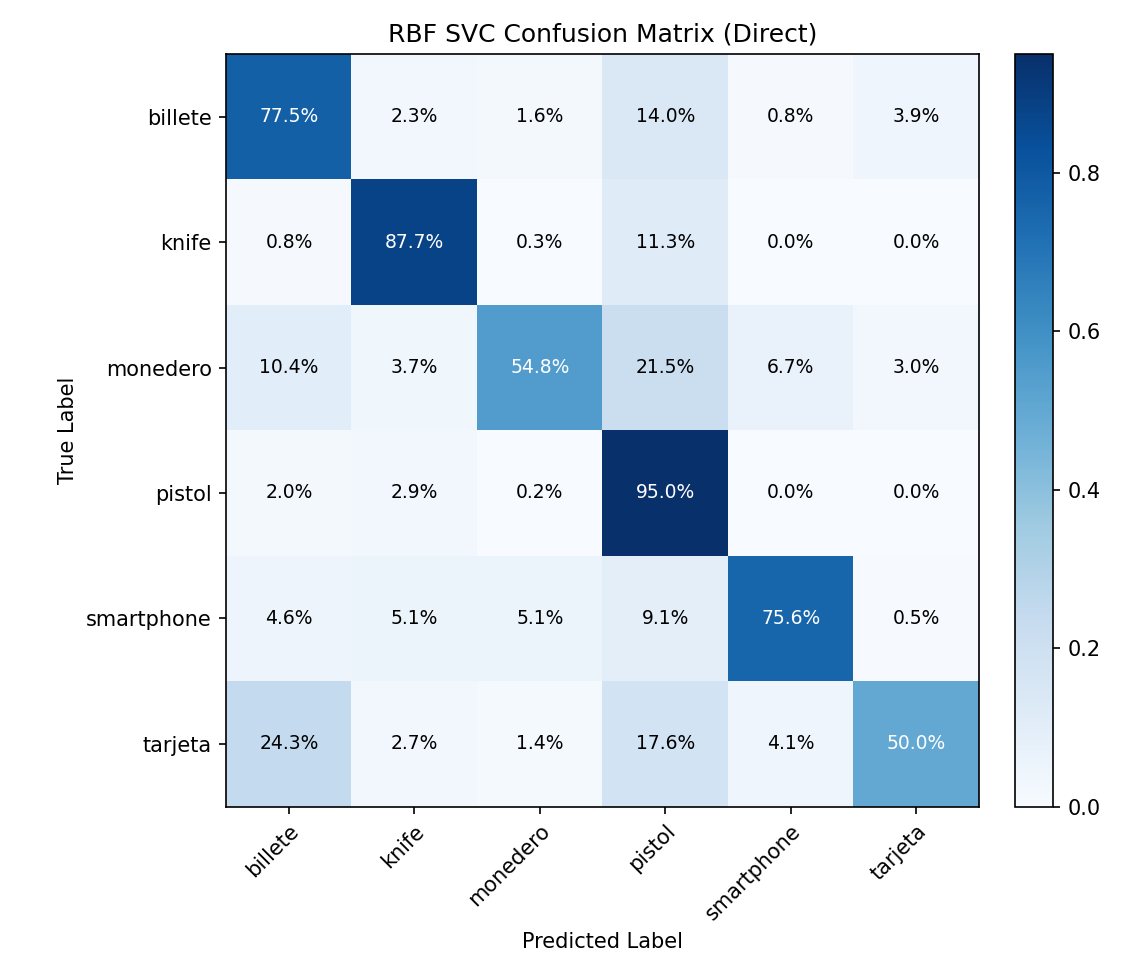
\includegraphics[width=\textwidth]{confusion_matrix_rbf_direct.png}
    \caption{SVM RBF}
  \end{subfigure}
  \caption{Ma trận nhầm lẫn chuẩn hóa theo hàng của hai mô hình SVM trên tập test (nhánh \emph{direct})}
  \label{fig:cm_rbf}
\end{figure}

\subsection{Phân tích lỗi}

\paragraph{Nhầm lẫn giữa súng ngắn và dao.} Đây là cặp bị nhầm lẫn nhiều nhất ở SVM tuyến tính trên nhánh \emph{direct} và hồi quy logistic. SVM tuyến tính phân loại nhầm 72 ảnh dao thành súng ngắn và 64 ảnh súng ngắn thành dao, chiếm 136 trong 447 lỗi (30\%). Với hồi quy logistic, số lỗi tương ứng là 55 và 69, chiếm 124 trong 512 lỗi (24\%). Một số ảnh của hai lớp có cạnh thẳng và vùng bàn tay che tương tự nhau.

\paragraph{Đồ vật thông thường bị phân loại thành súng ngắn.} Với SVM RBF, tỷ lệ ảnh bị phân loại thành \texttt{pistol} lần lượt là 21,5\% ở lớp ví, 17,6\% ở lớp thẻ ngân hàng, 14,0\% ở lớp tiền giấy và 9,1\% ở lớp điện thoại (Hình~\ref{fig:cm_rbf}, phần b). Trong bốn lớp này, ảnh ví có tỷ lệ bị phân loại thành súng ngắn cao nhất.

\paragraph{Thẻ ngân hàng bị phân loại thành tiền giấy.} SVM RBF phân loại 24,3\% ảnh thẻ ngân hàng thành tiền giấy. Hai loại vật thể có thể cùng xuất hiện dưới dạng hình chữ nhật với hoa văn bên trong. Báo cáo chưa đánh giá liệu đặc trưng màu sắc có giúp giảm nhầm lẫn giữa hai lớp này hay không.

\subsection{Thảo luận}
\label{sec:discussion}

\paragraph{Ảnh hưởng của cách chuẩn hóa kích thước.} Nhóm đặt ra hai giả thuyết để giải thích vì sao nhánh \emph{direct} đạt macro-F1 cao hơn nhánh \emph{padding} trong các thí nghiệm SVM.
\begin{itemize}
  \item \textbf{Phần ảnh chứa nội dung chiếm ít ô HOG hơn.} Với ảnh có tỷ lệ khung lớn hơn 2 hoặc nhỏ hơn 0,5, nội dung ảnh sau khi giữ tỷ lệ chiếm chưa đến một nửa khung hình vuông nếu bỏ qua sai số làm tròn. Các ô nằm hoàn toàn trong vùng đệm đồng nhất có gradient bằng 0, nên nội dung ảnh được biểu diễn bằng ít ô hơn so với khi co giãn trực tiếp.
  \item \textbf{Biến dạng có thể lặp lại trong cùng một lớp.} Nếu các ảnh cùng lớp có tỷ lệ khung tương tự, co giãn trực tiếp có thể tạo ra các biến dạng tương tự. Trong trường hợp đó, mô hình vẫn có thể học từ cấu trúc cạnh sau khi co giãn.
\end{itemize}
Có thể kiểm tra giả thuyết thứ nhất bằng cách so sánh chênh lệch giữa hai nhánh theo từng khoảng tỷ lệ khung ảnh.

\paragraph{Đối chiếu với mục tiêu ban đầu.}
\begin{itemize}
  \item \textbf{So sánh hai họ mô hình.} Nhóm đánh giá SVM và hồi quy logistic trên cùng một cách chia dữ liệu. Ba cấu hình được đối chiếu trên nhánh \emph{padding}.
  \item \textbf{Chọn chỉ số đánh giá.} Nhóm dùng macro-F1 để so sánh các cấu hình trên tập validation và báo cáo thêm kết quả theo lớp trên tập test.
  \item \textbf{Tinh chỉnh siêu tham số.} Nhóm khảo sát $C$ cho SVM tuyến tính và các tổ hợp $C$, $\gamma$ cho SVM RBF. Giá trị $C$ có điểm cao nhất của SVM tuyến tính nằm ở biên dưới của dải khảo sát. Hồi quy logistic dùng $C$ cố định.
  \item \textbf{Lựa chọn đặc trưng.} Với $C = 1$, các biến thể dùng ANOVA, kể cả khi kết hợp L1, đều có macro-F1 trên tập validation thấp hơn mô hình dùng toàn bộ đặc trưng.
\end{itemize}

\paragraph{Ảnh hưởng của điều chuẩn.} Chênh lệch macro-F1 giữa tập train và tập validation cho thấy dấu hiệu quá khớp ở hồi quy logistic. Vì nhóm giữ $C = 1$ trong cả năm biến thể, ảnh hưởng của mức điều chuẩn chưa được đánh giá riêng. Có thể khảo sát $C$ cho mô hình cơ sở trước, sau đó đối chiếu với các biến thể lựa chọn đặc trưng.

\paragraph{Khả năng mô hình dựa vào dấu hiệu ngoài hình dạng.} Tỷ lệ ảnh phải phóng to là 60\% ở lớp súng ngắn, 62\% ở lớp dao và 23\% ở lớp điện thoại. Nếu phép phóng to làm thay đổi độ sắc của cạnh, mô hình có thể sử dụng dấu hiệu này để phân loại. Một hướng kiểm tra là so sánh kết quả trong từng lớp giữa nhóm ảnh phải phóng to và nhóm ảnh còn lại.
